%%
%% This is file `sample-sigconf.tex',
%% generated with the docstrip utility.
%%
%% The original source files were:
%%
%% samples.dtx  (with options: `sigconf')
%% 
%% IMPORTANT NOTICE:
%% 
%% For the copyright see the source file.
%% 
%% Any modified versions of this file must be renamed
%% with new filenames distinct from sample-sigconf.tex.
%% 
%% For distribution of the original source see the terms
%% for copying and modification in the file samples.dtx.
%% 
%% This generated file may be distributed as long as the
%% original source files, as listed above, are part of the
%% same distribution. (The sources need not necessarily be
%% in the same archive or directory.)
%%
%%%% Proceedings format for most of ACM conferences (with the exceptions listed below) and all ICPS volumes.
\documentclass[sigconf,nonacm,11pt]{acmart}
%%%% As of March 2017, [siggraph] is no longer used. Please use sigconf (above) for SIGGRAPH conferences.

%%%% Proceedings format for SIGPLAN conferences 
% \documentclass[sigplan, anonymous, review]{acmart}

%%%% Proceedings format for SIGCHI conferences
% \documentclass[sigchi, review]{acmart}

%%%% To use the SIGCHI extended abstract template, please visit
% https://www.overleaf.com/read/zzzfqvkmrfzn

%%
%% \BibTeX command to typeset BibTeX logo in the docs
\AtBeginDocument{%
  \providecommand\BibTeX{{%
    \normalfont B\kern-0.5em{\scshape i\kern-0.25em b}\kern-0.8em\TeX}}}

\graphicspath{{fig/}{./}}

%%TC:ignore
%% Rights management information.  This information is sent to you
%% when you complete the rights form.  These commands have SAMPLE
%% values in them; it is your responsibility as an author to replace
%% the commands and values with those provided to you when you
%% complete the rights form.
\copyrightyear{2019}
\acmYear{2019}
\setcopyright{rightsretained}

%% These commands are for a PROCEEDINGS abstract or paper.
\acmConference{CSE6242}
\acmDOI{Data and Visual Analytics}
\acmISBN{}
\acmBooktitle{}
%%TC:endignore

%%
%% Submission ID.
%% Use this when submitting an article to a sponsored event. You'll
%% receive a unique submission ID from the organizers
%% of the event, and this ID should be used as the parameter to this command.
%%\acmSubmissionID{123-A56-BU3}

%%
%% The majority of ACM publications use numbered citations and
%% references.  The command \citestyle{authoryear} switches to the
%% "author year" style.
%%
%% If you are preparing content for an event
%% sponsored by ACM SIGGRAPH, you must use the "author year" style of
%% citations and references.
%% Uncommenting
%% the next command will enable that style.
%%\citestyle{acmauthoryear}

%%
%% end of the preamble, start of the body of the document source.
\begin{document}

%%
%% The "title" command has an optional parameter,
%% allowing the author to define a "short title" to be used in page headers.
\title{Evaluating Household Debt}

%%
%% The "author" command and its associated commands are used to define
%% the authors and their affiliations.
%% Of note is the shared affiliation of the first two authors, and the
%% "authornote" and "authornotemark" commands
%% used to denote shared contribution to the research.

%%TC:ignore
\author{George I. Kaveladze, Jason I. Chavez, John H. Tang, Khwala A. Abdulgader, Oluwagbemiga M. Adeosun}
\email{{gkaveladze3, jchavez8, jtang338, kabdulgader3, oadeosun7}@gatech.edu}
\affiliation{%
}

% \author{John Smith}
% \affiliation{\institution{The Th{\o}rv{\"a}ld Group}}
% \email{jsmith@affiliation.org}

% \author{Julius P. Kumquat}
% \affiliation{\institution{The Kumquat Consortium}}
% \email{jpkumquat@consortium.net}
%%TC:endignore

%%
%% By default, the full list of authors will be used in the page
%% headers. Often, this list is too long, and will overlap
%% other information printed in the page headers. This command allows
%% the author to define a more concise list
%% of authors' names for this purpose.
%%TC:ignore
%%\renewcommand{\shortauthors}{Tobin, et al.}
%%TC:endignore

%%
%% The abstract is a short summary of the work to be presented in the
%% article.
\begin{abstract}

The ability to accurately predict economic expansion or contraction is shown to be heavily reliant on household debt.  The correlation between economic downturns and high household debt levels is high, with household debt to GDP ratios having slightly higher predictive power.  Our household debt dashboard will provide users with the ability to observe the effects that changes in economic factors has on household debt and economic health, by proxy.  This approach will differentiate itself by predicting a factor that plays a large role in economic health, rather than attempting to predict economic health as a whole, allowing the model to account for more nuanced prediction factors.\vspace{-0.5em}

\end{abstract}

%%
%% The code below is generated by the tool at http://dl.acm.org/ccs.cfm.
%% Please copy and paste the code instead of the example below.
%%
%%TC:ignore
% \begin{CCSXML}
% <ccs2012>
%  <concept>
%   <concept_id>10010520.10010553.10010562</concept_id>
%   <concept_desc>Computer systems organization~Embedded systems</concept_desc>
%   <concept_significance>500</concept_significance>
%  </concept>
%  <concept>
%   <concept_id>10010520.10010575.10010755</concept_id>
%   <concept_desc>Computer systems organization~Redundancy</concept_desc>
%   <concept_significance>300</concept_significance>
%  </concept>
%  <concept>
%   <concept_id>10010520.10010553.10010554</concept_id>
%   <concept_desc>Computer systems organization~Robotics</concept_desc>
%   <concept_significance>100</concept_significance>
%  </concept>
%  <concept>
%   <concept_id>10003033.10003083.10003095</concept_id>
%   <concept_desc>Networks~Network reliability</concept_desc>
%   <concept_significance>100</concept_significance>
%  </concept>
% </ccs2012>
% \end{CCSXML}

% \ccsdesc[500]{Computer systems organization~Embedded systems}
% \ccsdesc[300]{Computer systems organization~Redundancy}
% \ccsdesc{Computer systems organization~Robotics}
% \ccsdesc[100]{Networks~Network reliability}

%%
%% Keywords. The author(s) should pick words that accurately describe
%% the work being presented. Separate the keywords with commas.
\keywords{Datasets, Household Debt, Economic Visualization, Household Debt to GDP Ratio, GDP Ratio, Interest Rate\vspace{-0.79em}}
%%TC:endignore

%% A "teaser" image appears between the author and affiliation
%% information and the body of the document, and typically spans the
%% page.
% \begin{teaserfigure}
%   \includegraphics[width=\textwidth]{sampleteaser}
%   \caption{Seattle Mariners at Spring Training, 2010.}
%   \Description{Enjoying the baseball game from the third-base
%   seats. Ichiro Suzuki preparing to bat.}
%   \label{fig:teaser}
% \end{teaserfigure}
%%
%% This command processes the author and affiliation and title
%% information and builds the first part of the formatted document.
%%TC:ignore
\maketitle
%%TC:endignore
\section{Introduction}

The field of macroeconomics has produced a wide variety of research into the predictability of economic expansion and contraction. Interest in this research field has increased over the years with many recent recessions providing a swath of data that can be analyzed and evaluated to determine the level of predictive power. The Great Recession of 2008, for instance, highlighted a set of factors that could be used to predict economic fluctuations, including recessions and market corrections.  Household debt, for example, was shown to have a negative impact on the GDP despite providing a short-term stimulus\cite{Kim2016}.  Accurately predicting this value could provide insights into of economic fluctuations and financial instability associated with government policies and consumer spending.  Research conducted by Zabai\cite{Zabai2017} has indicated that there is a direct correlation between economic health and household debt. Our goal for this project is to provide an interactive dashboard that allows users to observe correlations between household debt and other economic factors, along with predicting household debt given user-determined values for factors like consumer price index and yields on US Treasury 10 year bonds.\\
Since a large and rapid increase in household debt points to economic slowdown\cite{Mian2018}, this information can help users understand the impact their spending habits have. Similarly, the ability to adjust values and see outcomes could help legislators better understand the impact their policies have on the economy\cite{Garber2018}.\vspace{-1em}

%%\section{Key Features}

%% The Household Debt Dashboard will allow users to observe and quickly discern correlative associations between household debt and major economic factors.  Users will have the opportunity to adjust certain factors and observe the consequences of these values through the output of our Machine Learning algorithm that displays the predicted household debt.  This information will be coupled with GDP levels to enhance the user's understanding of the macroeconomic effects their proposals have.  Lastly, our solution will provide a containerized solution that allows interested parties to load the development environment necessary to create new models and visualization.\vspace{-1em}

\section{Problem Definition}

When a decline in the economic activity has been observed for multiple consecutive months a recession is to be expected in the United States. This directly destabilizes households, small businesses, and large corporations. US policy makers will utilize stimulus packages to mitigate long-term consequences but a spike in the unemployment rate and defaults on mortgages still occurs in the near term. Recessions have been observed to follow a business cycle. The ability to predict when the next economic downturn will occur allows corporations and US policy makers to properly plan and prevent a greater negative impact to the economy. As previous research has indicated there is a strong correlation between economic downturns and a high household debt[11], our dashboard will allow users to observe the effects that changes in economic factors have on household debt and economic health, by proxy.  Users will have the opportunity to adjust certain factors and observe the consequences of these values through the output of our Machine Learning algorithm that displays the predicted household debt. \vspace{-1em}

\section{Survey}

Our dashboard will leverage several studies performed on the correlative effects of household debt and economic downturns.\\
\vspace{0.25em}

\textbf{Studying The Great Recession}\\
Many studies have been conducted to better understand the factors that lead to the 2008 recession, including Chakrabarti et al.'s evaluation of household debt and savings during the recession\cite{Chakrabarti2015}, Nyman et al.'s Machine Learning approach to understanding the great recession\cite{Nyman2018}, and Mian et al.'s observation of household leverage and the recession\cite{Mian2010}.  All articles show the high correlation between economic downturns and increased household debt. We've used these articles to back our belief in the utility of household debt to predict recessions.\\
\vspace{0.25em}

\textbf{Macroeconomic effects of Household Debt}\\
General evaluations of the macroeconomic effects have been outlined in great detail in papers like Alter et al.'s global perspective on household debt effects\cite{Alter2018}, Friedman's theory of the consumption function\cite{Friedman1957}, Kim's empirical analysis of the effects of household debt\cite{Kim2016}, Lombardi et al.'s evaluation of the real effects of household debt\cite{Lombardi2017}, Mian et al.'s observations on household debt and worldwide business cycles\cite{Mian2015}\cite{Mian2018}, and Filardo's assessment on  the reliability of prediction models\cite{Filardo1999}. Each of these articles provide a backing for the global reach our proposed predictions can have, and provide a solid background on which correlations should receive particular attention. We'll expand this information by including more concentrated variables that relate specifically to household debt.\\

\vspace{0.25em}
\textbf{Policy Impacts on Economies and Household Debt}\\
If the provided proof of the relation between household debt and economic health have provided justification for our dashboard, studies on legislative effects provide motivation for creating the dashboard.  Garber et al.'s study of Brazil's 2014 recession\cite{Garber2018} and Guggenheim Investments' look into the effects rate cuts will continue to have in the US economic health\cite{Guggenheim2019} provide a basis for which variables our dashboard will allow users to adjust.\\
\vspace{0.5em}

\textbf{Current State of Debt}\\
A major push to produce our dashboard has come from research that reveal household debt is steadily climbing.  From Li's evaluation on the economics of student loans\cite{Li2013}, to Mian et al.'s study on the household leverage crisis\cite{Mian2011} and Zabai's assessment on recent household debt developments\cite{Zabai2017}, we've come to realize how much household debt continues to grow.  Leveraging this information, we hope to reveal what factors might be leading to this troubling trend.

%%\section{Risks, Rewards, and Cost}

%%\subsection{Risks}

%%We need as many input variables added in our model in the short time frame of the project.  For each input variable we need a large dataset to maximize the predictive power of the machine learning algorithm. The risk of influencing major decisions based on a poor prediction carries a heavy consequence.  While our models might show favorable statistics (e.g. low R2 and Mean Squared Error values), there is always the risk that our models either overfit the data or are biased towards a certain outcome.  Since mitigation strategies often include increasing training data observations, we also run the risk of not having a diverse enough set of training data to model against. 

%%\subsection{Rewards}

%The payoff of a model that accurately predicts household debt and presents it in an intuitive dashboard is huge. As Mian et al. observed, "the larger the increase in household leverage prior to the recession, the more severe the subsequent recession."\cite{Mian2018}.  Providing this information could encourage lawmakers to move beyond hypothetical outcomes and observe data driven predictions of economic responses.\vspace{-1em}

%\subsection{Costs}
%We will use open source data and software so the cost will be minimal other than human capital.  Depending on the availability and arrangements of Georgia Tech cloud based resources, the cost to host our solution would be the only concern.
\section{Proposed Method}
The following sections outline the methodology we have taken to produce our application:.\vspace{-0.5em}

\subsection{Dashboard}
The Household Debt dashboard will provide a multi-faceted approach to understanding the effects that various factors have on how citizen's borrowing practices.  This will be accomplished by, first, allowing users to observe visualizations that convey the relations between a subset of factors and household debt.  A household debt increases have been shown to be directly correlated with economic health\cite{Mian2015}, these visualizations will allow users to better understand the contributions that this debt has on a macroeconomic level and help curb the significant growth in household debt\cite{Alter2018}.\\
Additionally, users will have the ability to adjust the values associated with these highly correlative factors and observe the resulting household debt predictions.  Our predictions will be presented both textually and graphically as we explore visualizations that demonstrate the prediction's relation to GDP.\vspace{-0.5em}

\subsection{Predictions}

In order to provide significant predictions, we will gather data from a variety of sources and evaluate variable importance for predicting household debt. We have collected 29 economic data variables and completed a correlation analysis using R.  While other models have been created using the random forest algorithm\cite{Nyman2018}, we compared predictions from multiple machine learning models and found that linear regression produced the best overall predictions.\vspace{-0.5em}

\subsection{Technologies}

The application's user interface is a responsive single page application (SPA) based on AngularJS and Bootstrap. The graphs were generated using D3.js for visualization. We wrote extensive Scala and Apache Spark code to clean, transform, and insert our data into a SQLite database. We then used Scala and Apache Spark to aggregate the data and export it to a csv file which was then used to train and test our Azure ML Studio algorithms. We containerized our solution using Docker to allow users to run our cleaned data for their own exploration. Our website will be hosted on Heroku and has a Node.js back-end. The web application makes REST API calls to the Azure ML Studio for predictions. Our web application is hosted at https://teamfed-project.herokuapp.com/\#/landingPage.  

We have designed our application so that it can be executed a local PC or on the cloud.  The options to run our application are listed below.
\vspace{0.5em}

\textbf{Development server (Local Run without Docker)}
\begin{itemize}
\item Start a command shell
\item Navigate to the webapp directory.
\item Run the command "npm install" 
\item Run the command "npm start"
\item Start a browser and navigate to

http://localhost:8080/\#/landingPage
\end{itemize}


\textbf{Docker server (Locally run latest code using Docker)}
\begin{itemize}
\item Launch a command shell
\item Navigate to the webapp directory
\item Run the command "docker build -t teamfed ."
\item Run the command "docker run -p 8080:8080 teamfed" 
\item  Launch a browser and navigate to 

http://localhost:8080/\#/landingPage
\end{itemize}

\vspace{0.5em}
\textbf{Deploy to Heroku (Prod Run)}
\begin{itemize}
\item Install the HerokuCLI from

https://devcenter.heroku.com/articles/heroku-cli
\item Run heroku login to create a session to your heroku account.
\item Now you can sign into Container Registry heroku container:login.
\item Run heroku container:push web -a teamfed-project to create a docker image and push it to our Heroku repository.
\item Run heroku container:release web -a teamfed-project to release the latest image and this will update the webapp.
\item Run heroku logs --tail -a teamfed-project to see the logs and output from interacting with the webapp.
\item Navigate to 

https://teamfed-project.herokuapp.com/\#/

landingPage and watch the as the logs change and acknowledge the interaction with the webapp.
\end{itemize}

\vspace{-0.5em}


\subsection{Innovations}

Our dashboard includes the following innovative approaches. Firstly, based on our extensive research, there is a limited amount of models focusing on predicting household debt only, even though it is a strong indicator to the economic health of the United States. Many financial institutions produce economic models using household debt as a primary variable, therefore we are going to focus on this specific variable rather than predict the larger economy. Secondly, we are trying to account for negative rates by using the German 10 year yield in our model. This will allow our model to include data that is typically not used in United States recession models as the data is unavailable, but provides a complete view to an economic downturn. Lastly, we are streamlining our dashboard by providing an API of our machine learning model to the front-end and having a Node.js back-end while containerizing our solution using Docker.\vspace{0.5em}


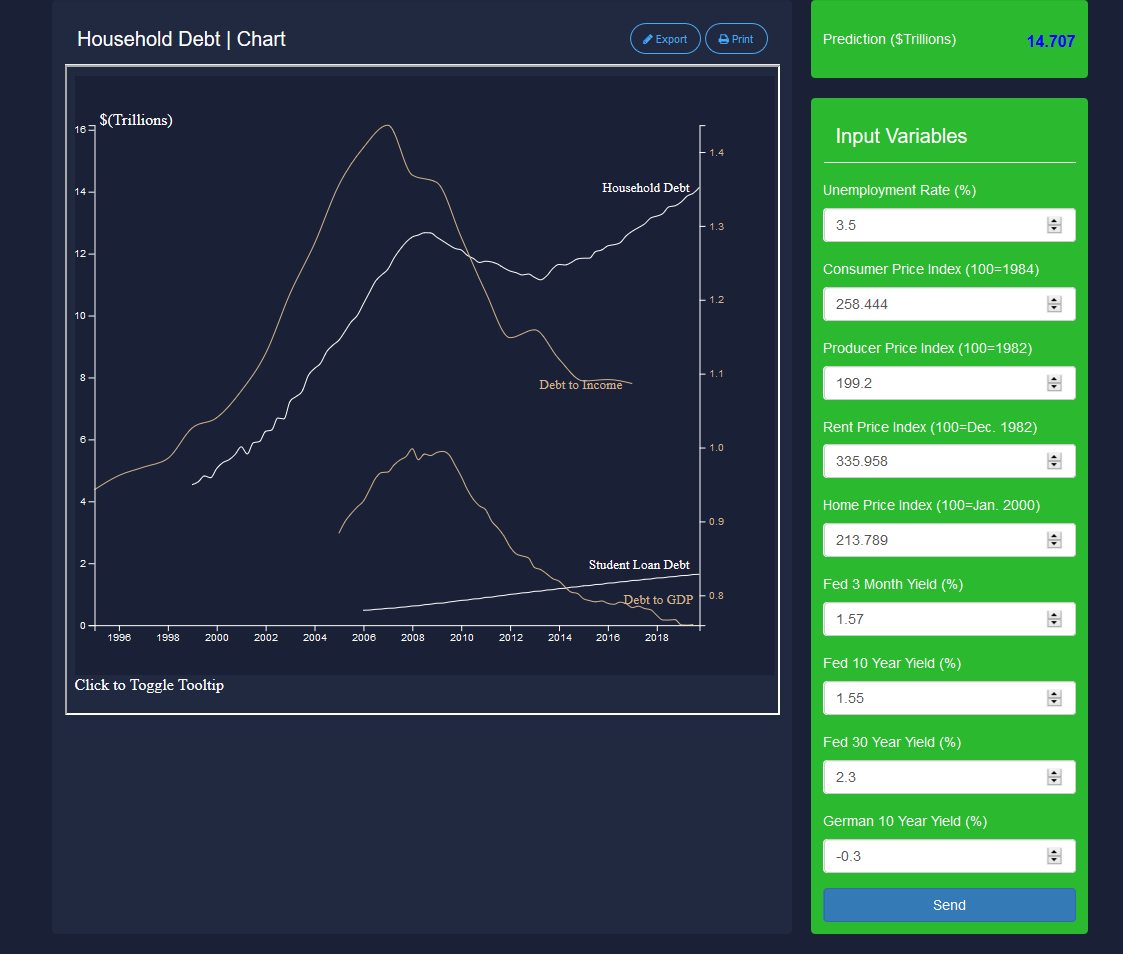
\includegraphics[scale = 0.32]{dashboard.png}
Figure 4.1 Responsive Web Application
\vspace{0.5em}

The top of our web application contains three buttons. The first two buttons are major components of household debt: GDP and student loan. They were eliminated as independent input variables during variable selection. They are major dependent parts of household debt. The user can click on the first two buttons to view visualizations of GDP and student loans, respectively. Clicking the last button will display the household debt along with debt to income, student loan, and debt to GDP.  

On the right side of the screen are text entry boxes for the Azure ML Studio's independent input variables. They default to data from the fourth quarter of 2019. The user can change the values as needed. Clicking on the Send button at the bottom of the screen will submit the form values, via a REST API call, to our model hosted at Microsoft Azure ML Studio. Our model will make a prediction and send it back to the web page.  The prediction will be displayed in the top text box.

\section{Experiments and Evaluation}
In order to validate our methodology when creating our household debt dashboard, we have compiled a list of steps that we have reviewed throughout our process. These steps are outlined as follows. Firstly, we have collected a large amount of data sets to determine which input variables will provide the highest predictive power. The data sets and their sources are listed in the Appendix under "Table 1 Data Sets". Secondly, we evaluated multiple machine learning algorithms: Bayesian Linear Regression, Linear Regression, Boosted Decision Tree, Decision Forest Regression, and Neural Network Regression. This ensured that our study utilized the most suitable methodology when predicting household debt. Thirdly, we have included a user interactivity feature as we believe allowing the user to enter various data elements will provide a greater understanding of the factors that impact household debt. Fourthly, we have researched various economic dashboard visualizations to ensure we compartmentalize the information in an intuitive manner for the user. Lastly, we believe our front-end and back-end methodology is stream-lined as stated in the innovations section above. 


We used R with the tidyverse, GGally, rpart, and caret libraries to help select the input variable with the highest prediction power for household debt. Our initial step in variable reduction was to evaluate variable correlation (both with the response variable and the predictor variables with one another).  To do so, we created a correlation matrix that was evaluated in the following ways:


\begin{itemize}

\item The correlation each variable has with the response variable (Household Debt).  We do this both visually and numerically, where the straighter the line visually, the higher the correlation value ought to be numerically

\item Correlation of each predictor variable to one another.  If a predictor variable is highly correlated with another variable, we needed to choose one of the two as to not over-weight the underlying data that both variables are explaining.

\end{itemize}

\vspace{0.5em}
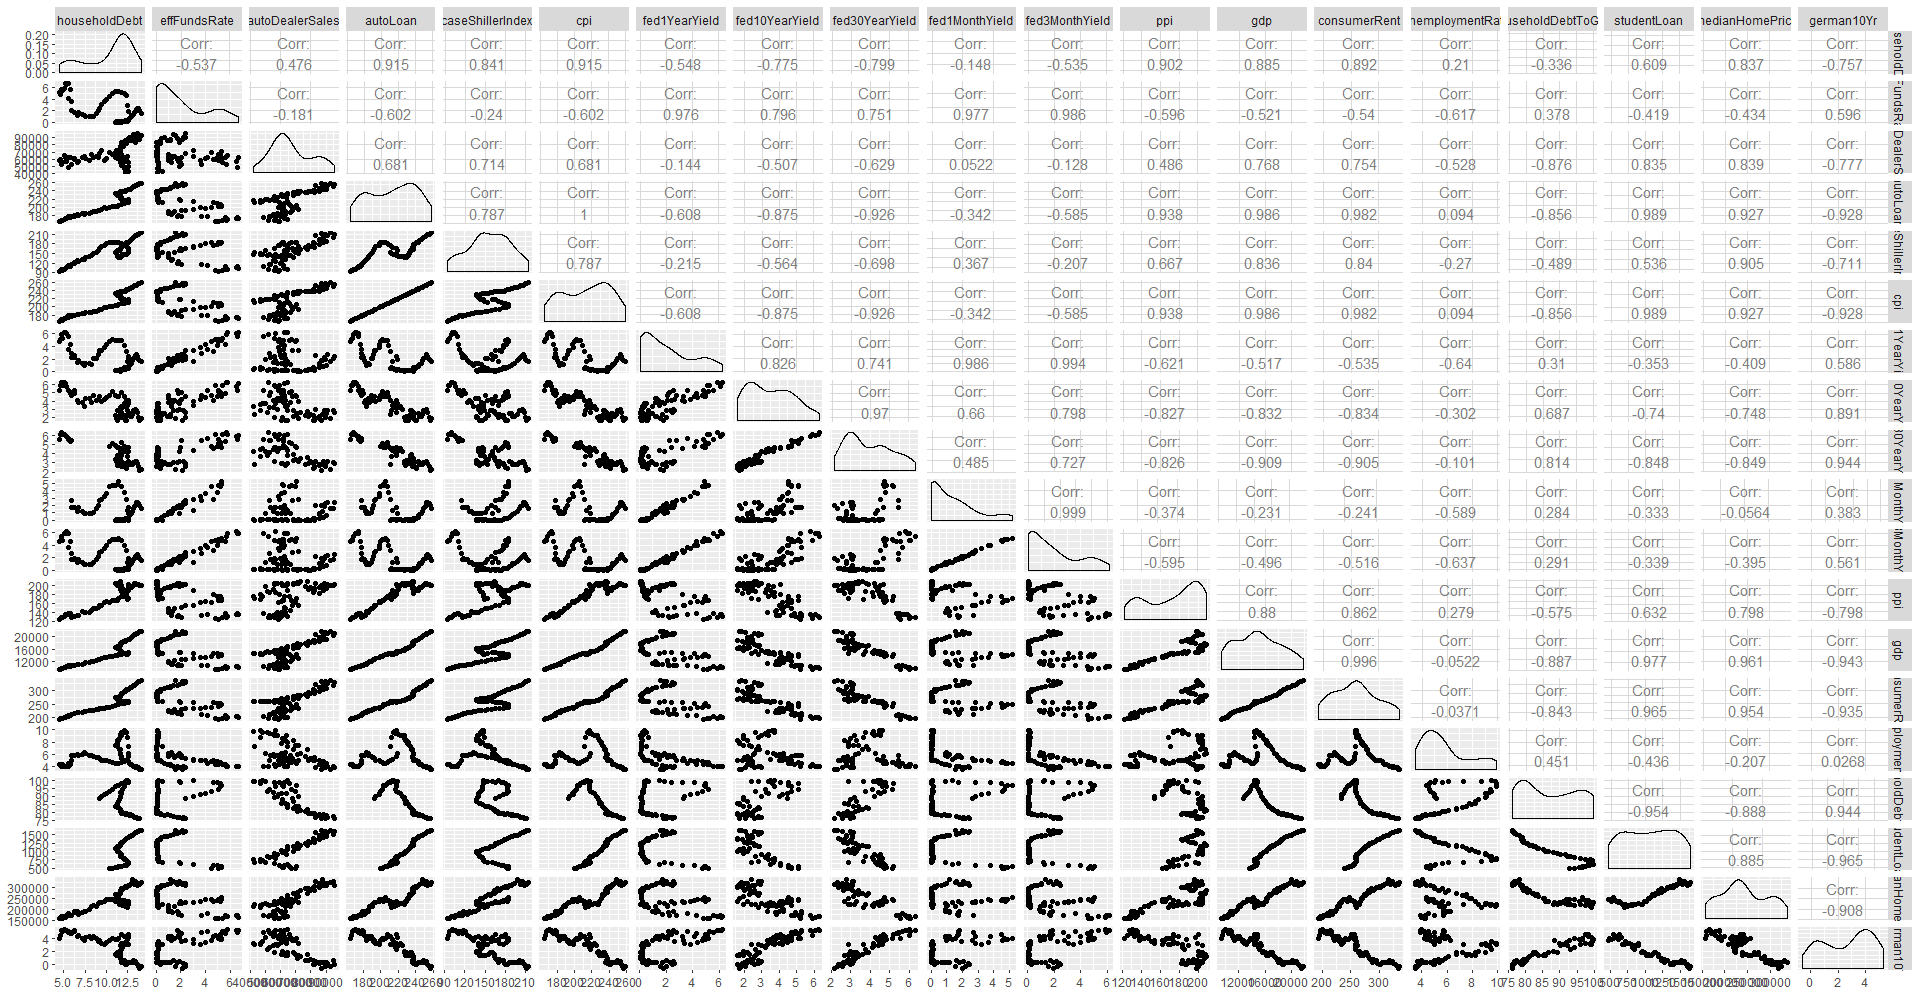
\includegraphics[scale = 0.12]{Correlation_Plot_All.png}

Figure 5.1 Correlation For All Input Variables
\vspace{0.75em}

We dropped input variables which had less than 0.75 correlation to household debt or if the ML model showed that an interaction of variables was highly predictive. As shown in the Figure 5.2, both the Fed 3 Month Yield and Unemployment Rate had low correlations, but the interaction they had with other variables improved the overall model score. Using this graph as a guide, we reduced the number of input variables from eighteen to just nine. Our final list of input variables are the consumer price index, Treasury 3 month bond yield, Treasury 10 year bond yield, Treasury 30 year bond yield, consumer rent, German 10 year bond yield, S&P Case Shiller Index, Producer Price Index, and the unemployment rate. Please see the appendix "Table 3. Correlation For Final Input Variables" for a larger correlation graph.


\vspace{0.5em}
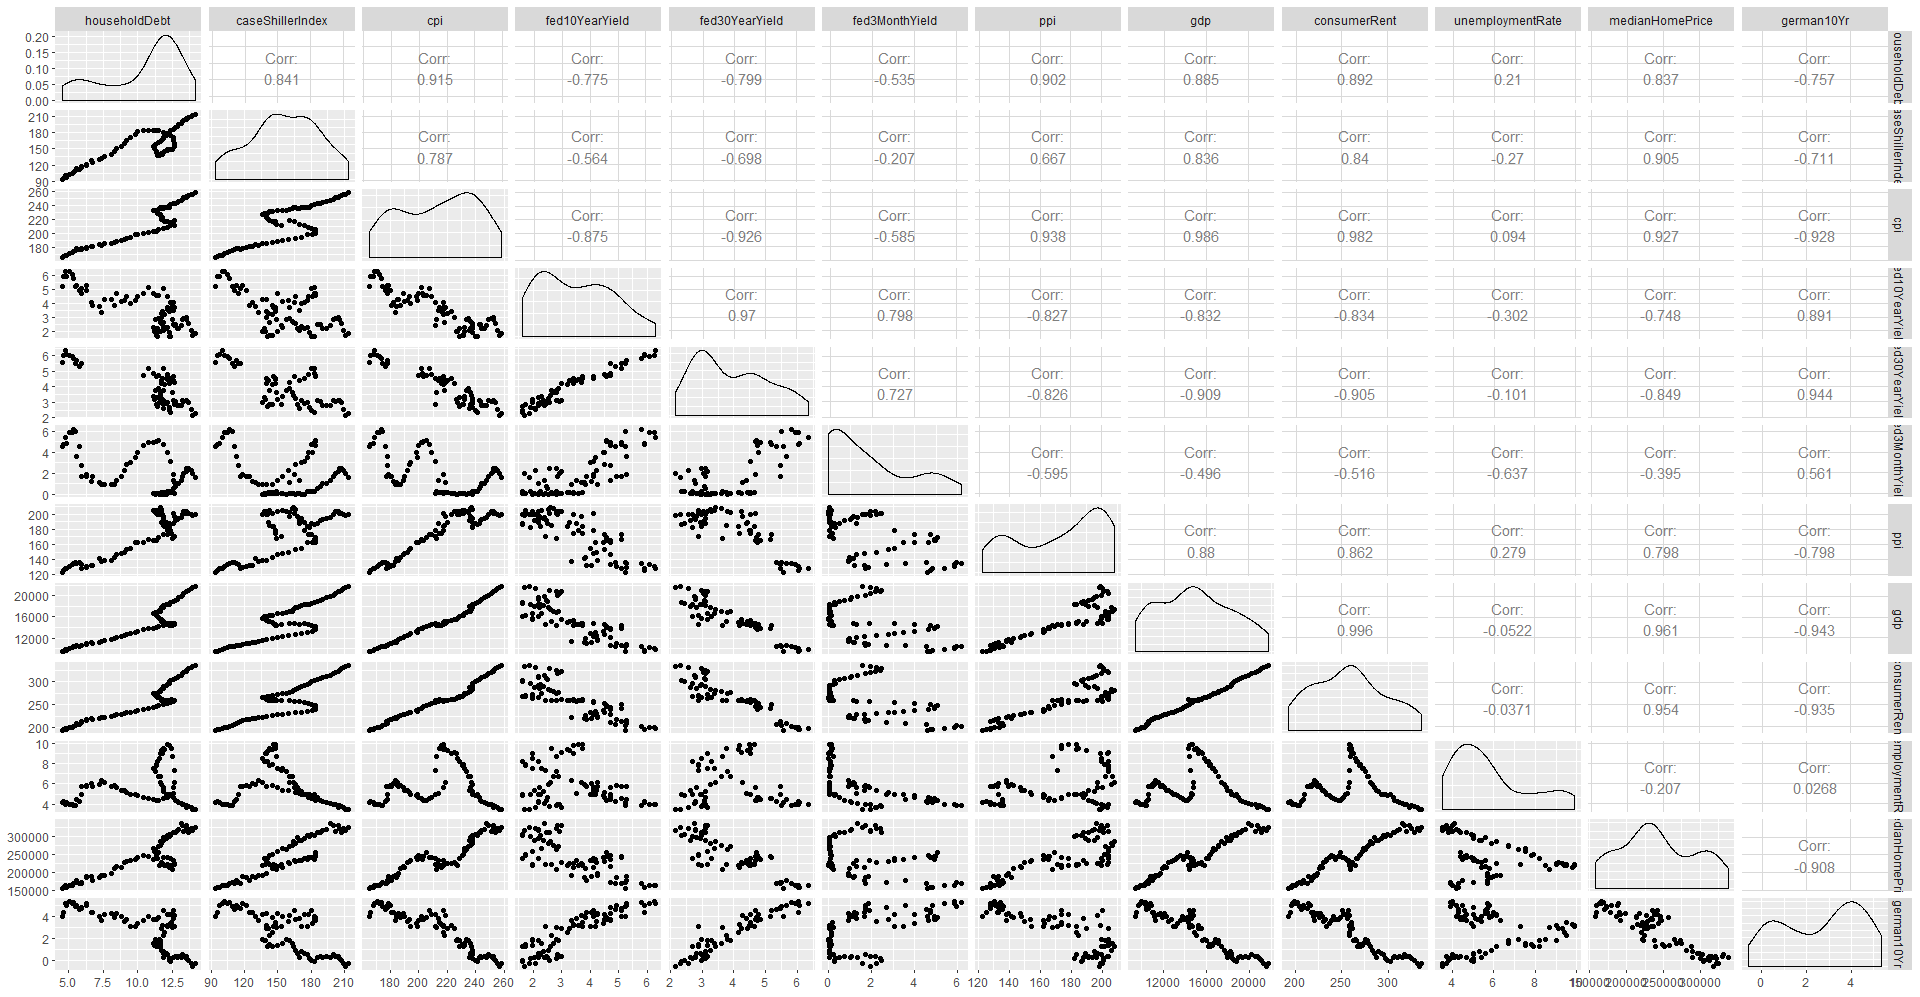
\includegraphics[scale = 0.13]{Correlation_Plot_Final.png}

Figure 5.2 Correlation For Final Input Variables
\vspace{1.25em}

\includegraphics[scale = 0.25]{linreg.png}
Figure 5.3 Prediction vs Final Input Variables and Actual Household Debt 
\vspace{1.0em}


We also had to determine what time scale our study should use. We had to decide if our model should predict household debt on a yearly, quarterly, or monthly basis. We were inspired by Nyman et al.'s Machine Learning approach to understanding the great recession\cite{Nyman2018} use of a quarterly time scale.  Their Random Forest model did a poor job on a daily and yearly scale but it worked quite well on a quarterly basis. Once we chose the proper time scale, we evaluated the scale to determine if there's enough of a difference in Household Debt per quarter to see if we should include the quarter as a variable.  As shown in the plot, each quarter's distribution closely matched that of the other quarters, meaning there would be negligible improvement in predictions.
 
 
\vspace{0.5em}
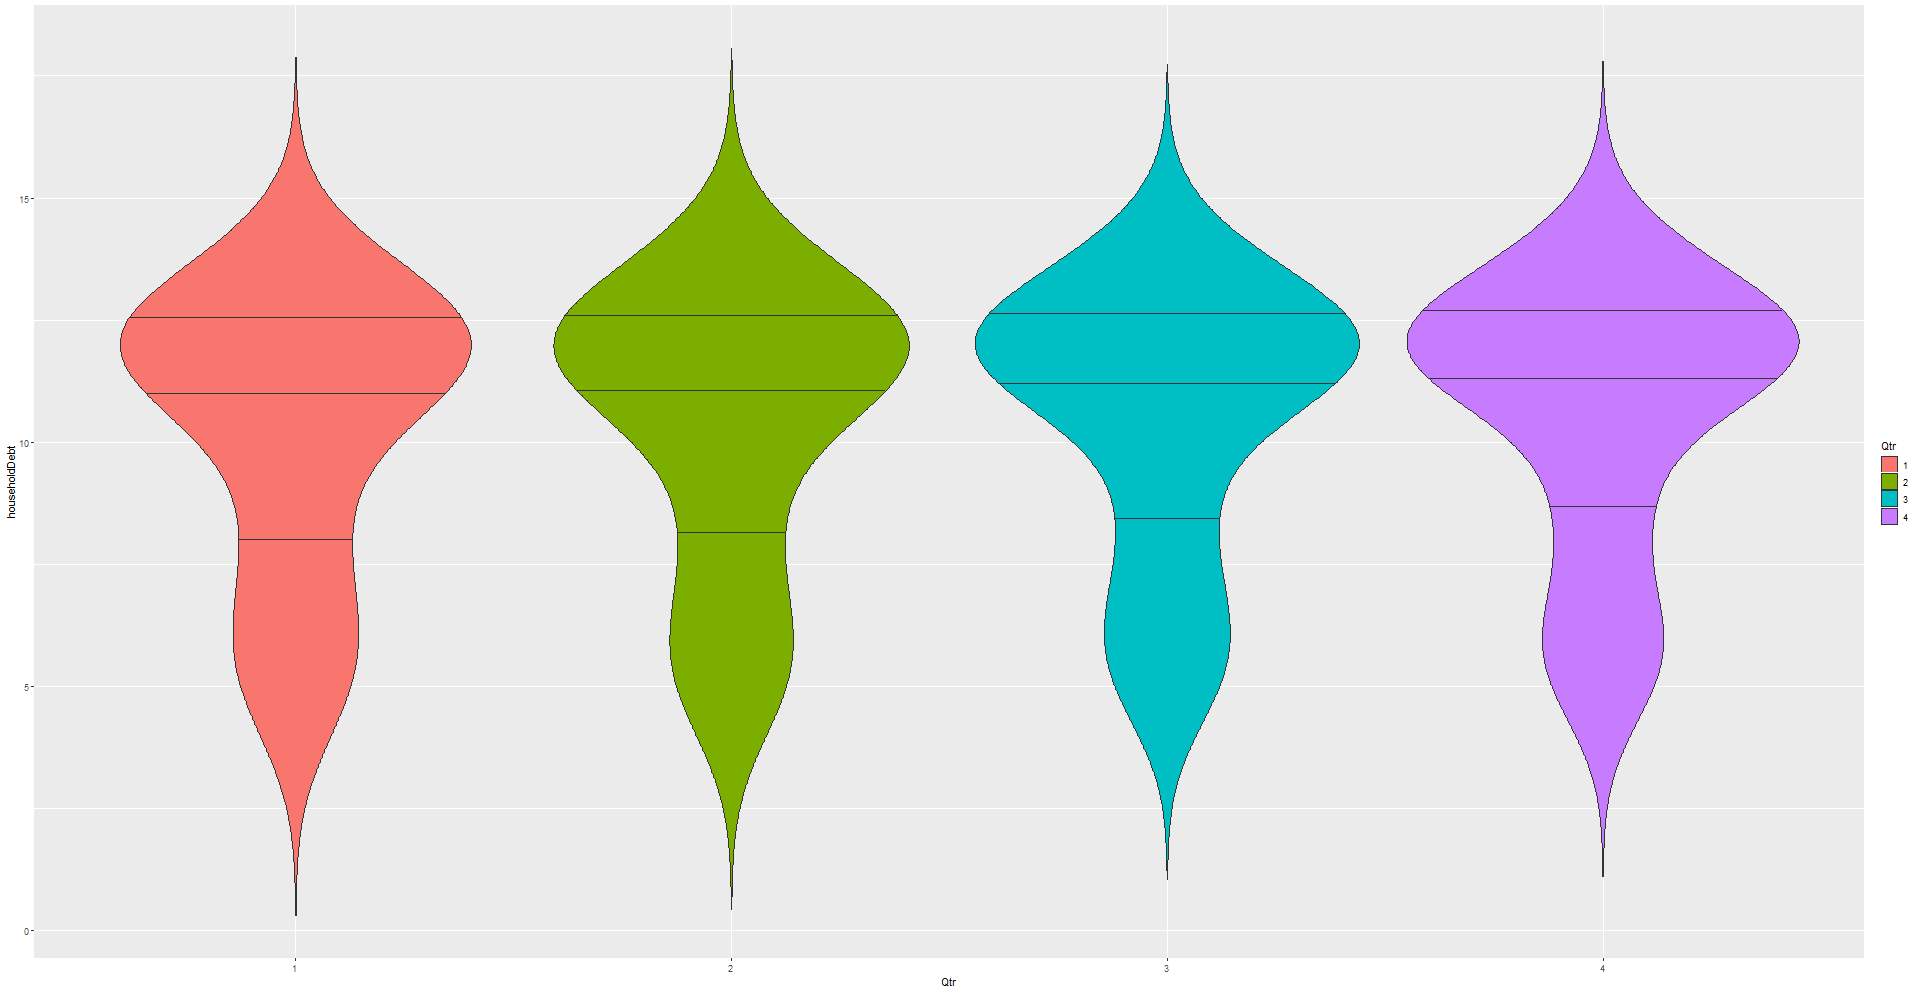
\includegraphics[scale = 0.13]{QtrVSHouseholdDebt_violinPlot.png}

Figure 5.4 Violin Plot of Debt On Quarterly Time Scale
\vspace{0.75em}

Another assessment we had to perform was the effectiveness of the number of input variables our study used. What number of variables would reduce the amount of reduction in Mean Squared Error (MSE)?  Figure 5.5 shows that there isn't much of a gain in LASSO regression once the model had more than 7 variables.  We ran two Linear Regression models with both 9 and 7 variables (removing the two lowest correlative variables) and found that 9 variables yielded the best statistics.


\vspace{0.5em}
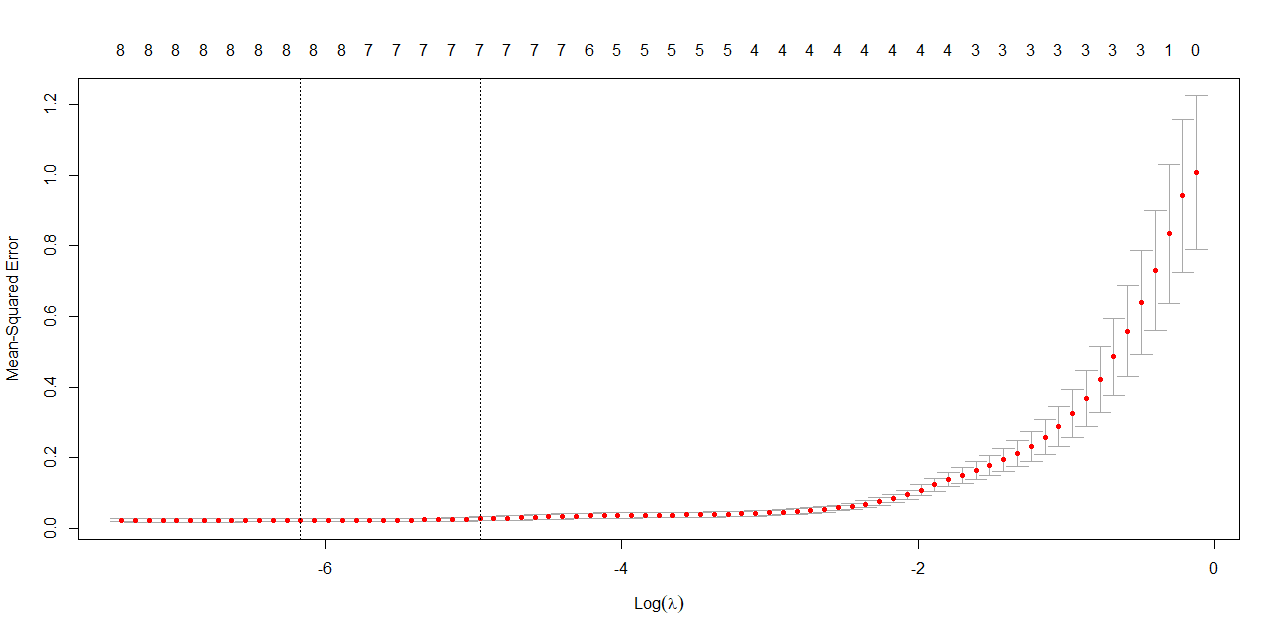
\includegraphics[scale = 0.18]{LASSORegression_Plot.png}

Figure 5.5 Lasso Regression Plot of Mean Squared Error vs Num of Input Variables
\vspace{0.75em}

One concern the group with the model was not accounting for the autocorrelation of Household Debt.  As shown in Figure 5.6, the autocorrelation of Household Debt is high in the first 3 quarters of a year.  However, attempting to split the data to allow this information to be incorporated in the model led to an overfitting of the model to the training dataset, so we decided not to account for this response variable characteristic.

\vspace{0.5em}
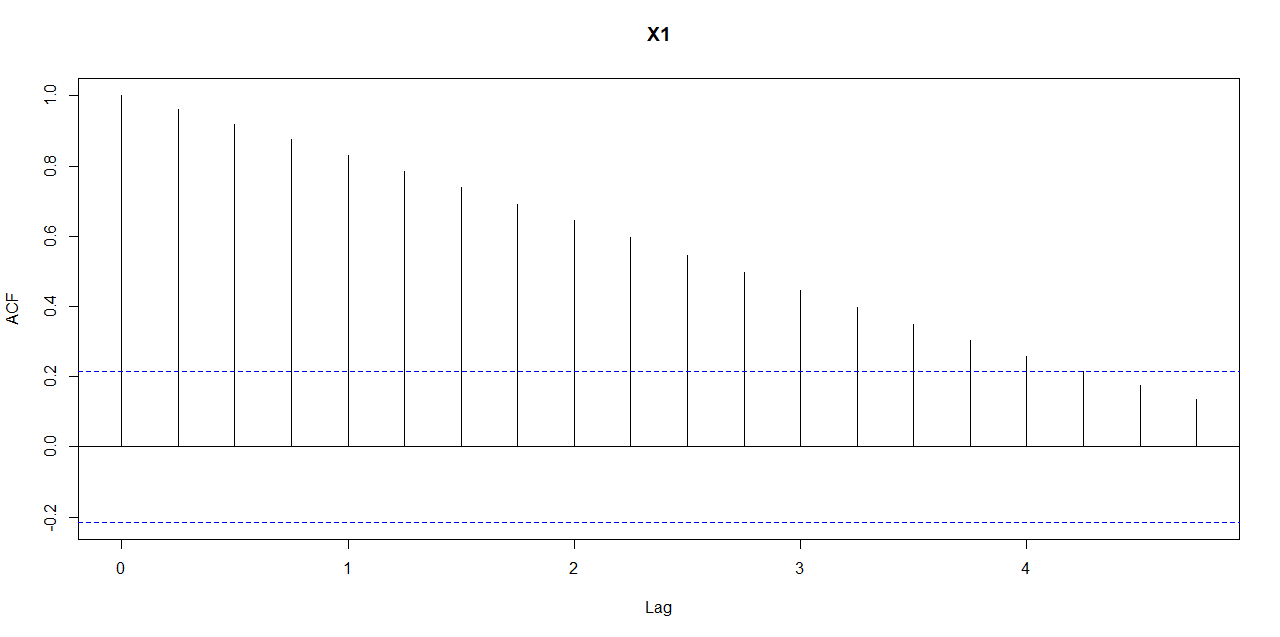
\includegraphics[scale = 0.18]{HouseholdDebtAutoCor.png}

Figure 5.6 Household Debt Auto Correlation
\vspace{0.75em}

We used a data split of 80 percent for training and 20 percent for testing. Our web application feeds the input variables to a Microsoft Azure Machine Learning algorithm using REST API calls. The calls are secured with a private key.  We were shocked as we got back the predictions.  We thought the more sophisticated machine learning algorithms such as Decision Forest Regression or Neural Network Regression would produce superior predictions. The two best models were the Neural Network Regression and the Linear Regression, with the difference between them being negligible.  As such, we decided to use the Linear model for our project as it's easiest to explain/understand.

\begin{center}
    \begin{tabular}{||c|c||}
    \hline
    Variable & Coefficient\\
    \hline\hline
    Bias & -.937356\\
    Fed 10 Yr Yield & -0.790002\\
    Fed 30 Yr Yield & 0.534679\\
    German 10 Yr Yield & 0.495695\\
    Unemployment Rate & 0.428106\\
    Consumer Price Index & -0.0940645\\
    Consumer Rent & 0.0798328\\
    Fed 3 Month Yield & 0.0515536\\
    Case Shiller Index & 0.0503518\\
    Producer Price Index & 0.047038\\
    \hline
    \end{tabular}
\end{center}

\begin{center} Figure 5.7 Model Coefficients \end{center}


Observing the model predictions in Figure 5.8, we see that the Linear Regression model using the variables displayed above closely predicts the Household Debt.

\includegraphics[scale = 0.34]{Final Predictions.png}
\begin{center}Figure 5.8 Final Prediction Comparison \end{center}

TO-DO: Need Final Web UI and write up

Please see the Appendix for information about the project's source code.

\section{Plan of Activities}

We achieved success by following the plan below:\vspace{0.07em}
\begin{center}
    \begin{tabular}{||c|c||}
    \hline
    Activity & Completion Date (03/27)\\
    \hline\hline
    Collect Data & 03/07\\
    Variable Exploration & 03/20\\
    Clean Data & 03/21\\
    Variable Selection & 03/27\\
    Progress Report & 03/27\\
    ML Algorithm Developed & 04/03\\
    Front-end Setup & 04/03\\
    Back-end Setup & 03/31\\
    Final Report & 04/13\\
    \hline
    \end{tabular}
\end{center}

\textbf{All group members have continued to contribute a similar amount of effort.} The following activities were completed by the following teammates: Data Collection: John and Khwala; Variable Exploration: George; Data Cleansing: John and Jason; Variable Selection: Jason and Khwala; ML Algorithm: Jason; Front-end Set Up: Bemi and George; Back-end Set Up: Bemi; Progress Report: Khwala; Final Report: Khwala, Jason, and John. 



\section{Conclusions and Discussion}


We intially started with 28 input variables. We knew that some of the variables were going to be eliminated during our variable selection phase. We were surprised that automobile loans, auto dealer sales, consumer rent, and student loans did not make the final list of input variables. 

Graphing and analyzing exisisting data provided a clear near term trend of household debt. We were not suprised when our model predicted ever increasing household debt for 2020. We were very worried about what this meant for the econonmy. The model predicted a household debt value that was far greater than the value from the last recession of 2008.  While we didn't know that the coronavirus would be the spark that would deflate the economy, our model clearly alerted us that the economy was going to tank.


%\section{Related Work}

%Our dashboard will leverage several studies performed on the correlative effects of household debt and economic downturns.\\
%\textbf{Studying The Great Recession}\\
%Many studies have been conducted to better understand the factors that lead to the 2008 recession, including Chakrabarti et al.'s evaluation of household debt and savings during the recession\cite{Chakrabarti2015}, Nyman et al.'s Machine Learning approach to understanding the great recession\cite{Nyman2018}, and Mian et al.'s observation of household leverage and the recession\cite{Mian2010}.  All articles show the high correlation between economic downturns and increased household debt, which we've used to back our belief in the utility of household debt predictions and will leverage to evaluate variable importance.\\
%\textbf{Macroeconomic effects of Household Debt}\\
%General evaluations of the macroeconomic effects have been outlined in great detail in papers like Alter et al.'s global perspective on household debt effects\cite{Alter2018}, Friedman's theory of the consumption function\cite{Friedman1957}, Kim's empirical analysis of the effects of household debt\cite{Kim2016}, Lombardi et al.'s evaluation of the real effects of household debt\cite{Lombardi2017}, Mian et al.'s observations on household debt and worldwide business cycles\cite{Mian2015}\cite{Mian2018}, and Filardo's assessment on  the reliability of prediction models\cite{Filardo1999}. Each of these articles provide a backing for the global reach our proposed predictions can have, and provide a solid background on which correlations should receive particular attention. We'll expand this information by including more concentrated variables that relate specifically to household debt.\\
%\textbf{Policy Impacts on Economies and Household Debt}\\
%If the provided proof of the relation between household debt and economic health have provided justification for our dashboard, studies on legislative effects provide motivation for creating the dashboard.  Garber et al.'s study of Brazil's 2014 recession\cite{Garber2018} and Guggenheim Investments' look into the effects rate cuts will continue to have in the US economic health\cite{Guggenheim2019} provide a basis for which variables our dashboard will allow users to adjust.\\
%\textbf{Current State of Debt}\\
%A major push to produce our dashboard has come from research that reveal household debt is steadily climbing.  From Li's evaluation on the economics of student loans\cite{Li2013}, to Mian et al.'s study on the household leverage crisis\cite{Mian2011} and Zabai's assessment on recent household debt developments\cite{Zabai2017}, we've come to realize how much household debt continues to grow.  Leveraging this information, we hope to reveal what factors might be leading to this troubling trend.

\bibliographystyle{ACM-Reference-Format}
\bibliography{reference}

%%
%% If your work has an appendix, this is the place to put it.
\appendix
\begin{appendix}

\section{Appendix}
\label{appendix:datasets}




\begin{table*}[ht]
\caption{Data Sets}
\centering
\begin{tabular}{p{0.05\linewidth}p{0.35\linewidth}p{0.6\linewidth}}
\hline
Num & Description & Source\\
\hline
1 & 1 Month Treasury & https://fred.stlouisfed.org/series/GS1M\\
2 & 3 Month Treasury & https://fred.stlouisfed.org/series/GS3M\\
3 & 1 Year Treasury & https://fred.stlouisfed.org/series/GS10\\
4 & 10 Year Treasury & https://fred.stlouisfed.org/series/GS10\\
5 & 30 Year Treasury & https://fred.stlouisfed.org/series/GS30\\
6 & 10 Year Real Rates & https://fred.stlouisfed.org/series/FII10\\
7 & Automobile Loans & https://fred.stlouisfed.org/series/CARACBW027SBOG\\
8 & Auto Dealer Sales & https://fred.stlouisfed.org/series/MRTSSM4411USN\\
9 & Consumer Price Index & https://fred.stlouisfed.org/series/CPIAUCSL\\
10 & County Codes & https://data.bls.gov/cew/doc/titles/area/area\_titles.htm\\
11 & Credit Card Rate & https://fred.stlouisfed.org/series/TERMCBCCINTNS\\
12 & Employee Cost Index & https://data.bls.gov/cgi-bin/surveymost?bls\\
13 & Fed Effective Funds Rate  & https://fred.stlouisfed.org/series/DFF\\
14 & German 10 Year Yield & https://fred.stlouisfed.org/series/IRLTLT01DEM156N\\
15 & Household Debt & https://www.newyorkfed.org/medialibrary/media/research/\\
 & & national\_economy/householdcredit/pre2003\_data.xlsx\\ 
 & & and\\
 & & https://www.newyorkfed.org/medialibrary/interactives/householdcredit/\\
 & & data/xls/hhd\_c\_report\_2019q4.xlsx\\
16 & Household Debt to Income By County & https://www.federalreserve.gov/releases/z1/dataviz/household\_debt/\\
17 & Household Debt to Income By State  & https://www.federalreserve.gov/releases/z1/dataviz/household\_debt/\\
18 & Household Debt to GDP & https://fred.stlouisfed.org/series/HDTGPDUSQ163N\\
19 & Median Home Prices & https://fred.stlouisfed.org/series/MSPUS\\
20 & Non Farm Employmment (NFE) & https://download.bls.gov/pub/time.series/ce/\\
 & & ce.data.00a.TotalNonfarm.Employment\\
21 & Produce Price Index  & https://fred.stlouisfed.org/series/PPIACO\\
22 & Rental Vacancy & https://fred.stlouisfed.org/series/RRVRUSQ156N\\
23 & S\&P/Case-Shiller Index & https://fred.stlouisfed.org/series/CSUSHPISA\\
24 & State Codes & https://www.bls.gov/respondents/mwr/electronic-data-interchange/appendix-d-usps-state-abbreviations-and-fips-codes.htm\\
25 & Student Loans & https://fred.stlouisfed.org/series/SLOAS\\
26 & Total Employee Compensation & https://data.bls.gov/pdq/SurveyOutputServlet\\
27 & Unemployment Rate & https://fred.stlouisfed.org/series/UNRATE/\\
28 & Urban Consumer Rent & https://fred.stlouisfed.org/series/CUSR0000SAS2RS\\
29 & U.S. GDP  & https://fred.stlouisfed.org/series/GDP\\
\hline
\end{tabular}
\end{table*}




\begin{table*}[ht]
\caption{Correlation Report For All Input Variables}
\centering
\begin{tabular}{p{1.0\linewidth}}
\hline
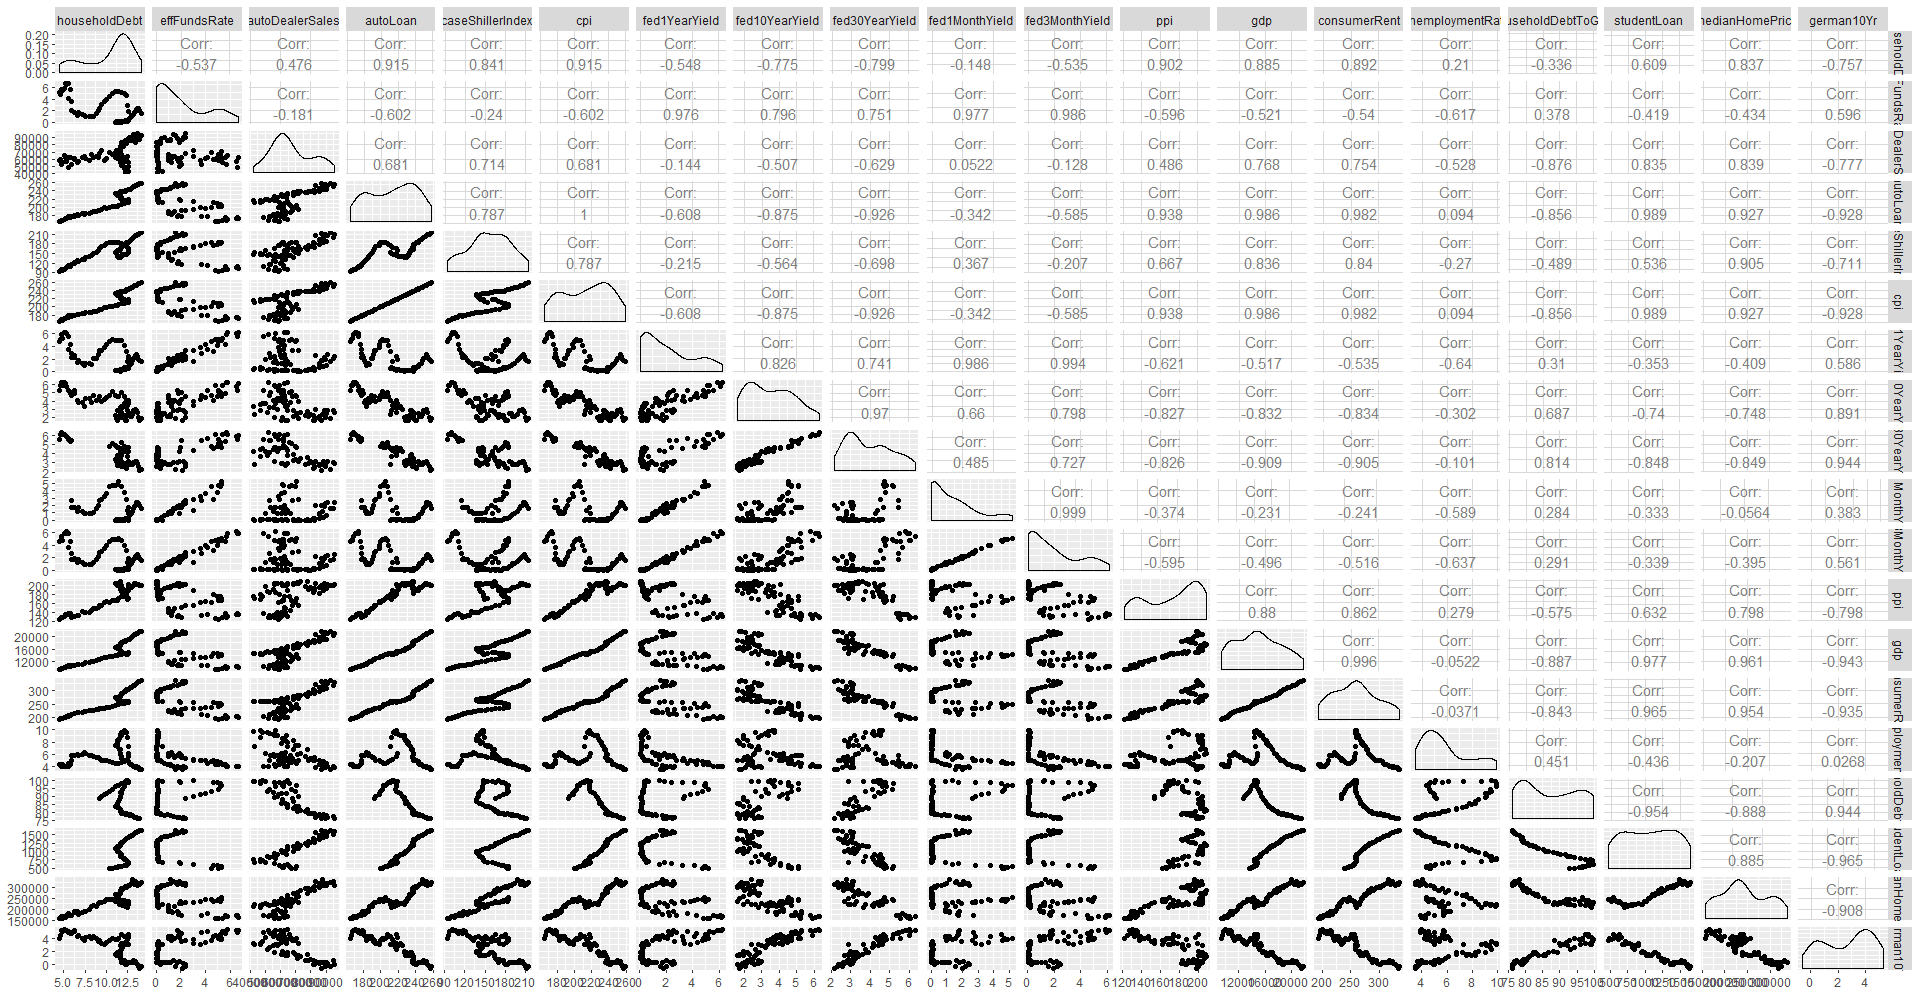
\includegraphics[scale = 0.27]{Correlation_Plot_All.png}\\
\hline
\end{tabular}
\end{table*}

\begin{table*}[ht]
\caption{Correlation Report For Final Input Variables}
\centering
\begin{tabular}{p{1.0\linewidth}}
\hline
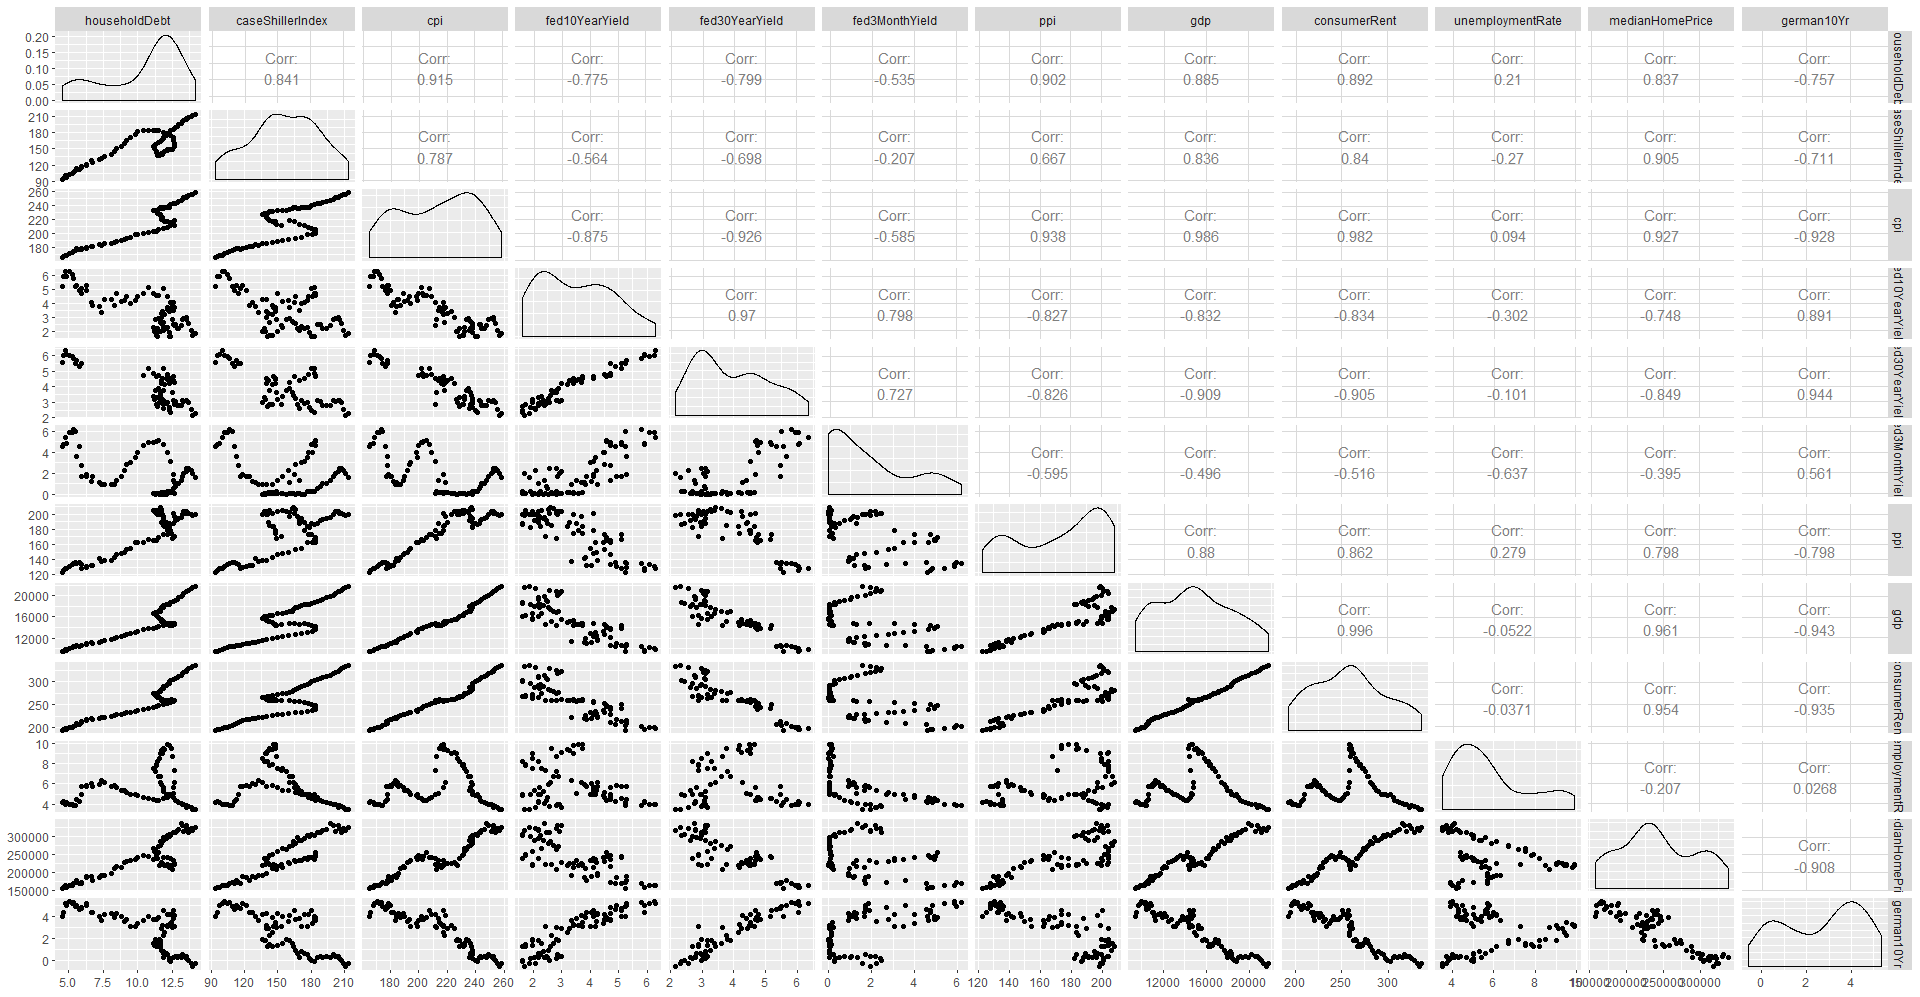
\includegraphics[scale = 0.27]{Correlation_Plot_Final.png}\\
\hline
\end{tabular}
\end{table*}

\begin{table*}[ht]
\caption{Prediction vs Final Input Variables and Actual Household Debt}
\centering
\begin{tabular}{p{1.0\linewidth}}
\hline
\includegraphics[scale = 0.27]{linreg.png}\\
\hline
\end{tabular}
\end{table*}


\begin{table*}[ht]
\caption{Violin Plot of Debt On Quarterly Time Scale}
\centering
\begin{tabular}{p{1.0\linewidth}}
\hline
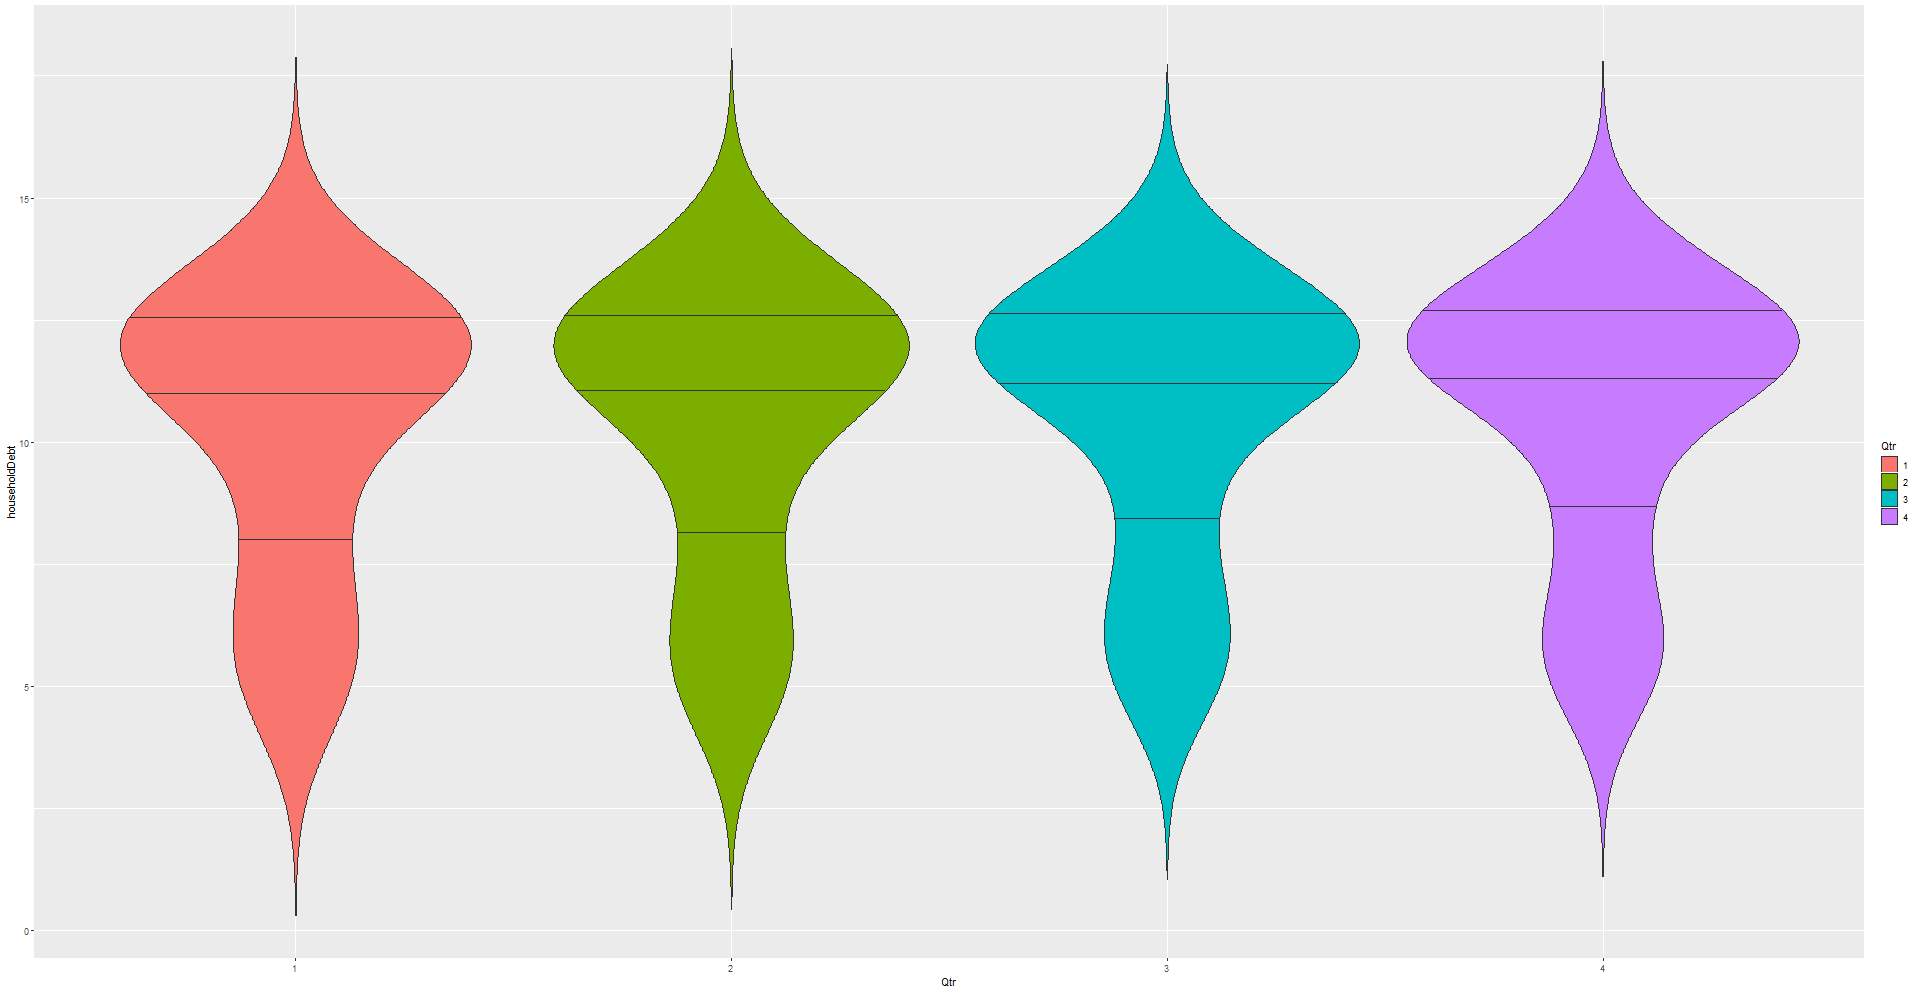
\includegraphics[scale = 0.26]{QtrVSHouseholdDebt_violinPlot.png}\\
\hline
\end{tabular}
\end{table*}

\begin{table*}[ht]
\caption{Lasso Regression Plot of Mean Squared Error vs Num of Input Variables}
\centering
\begin{tabular}{p{1.0\linewidth}}
\hline
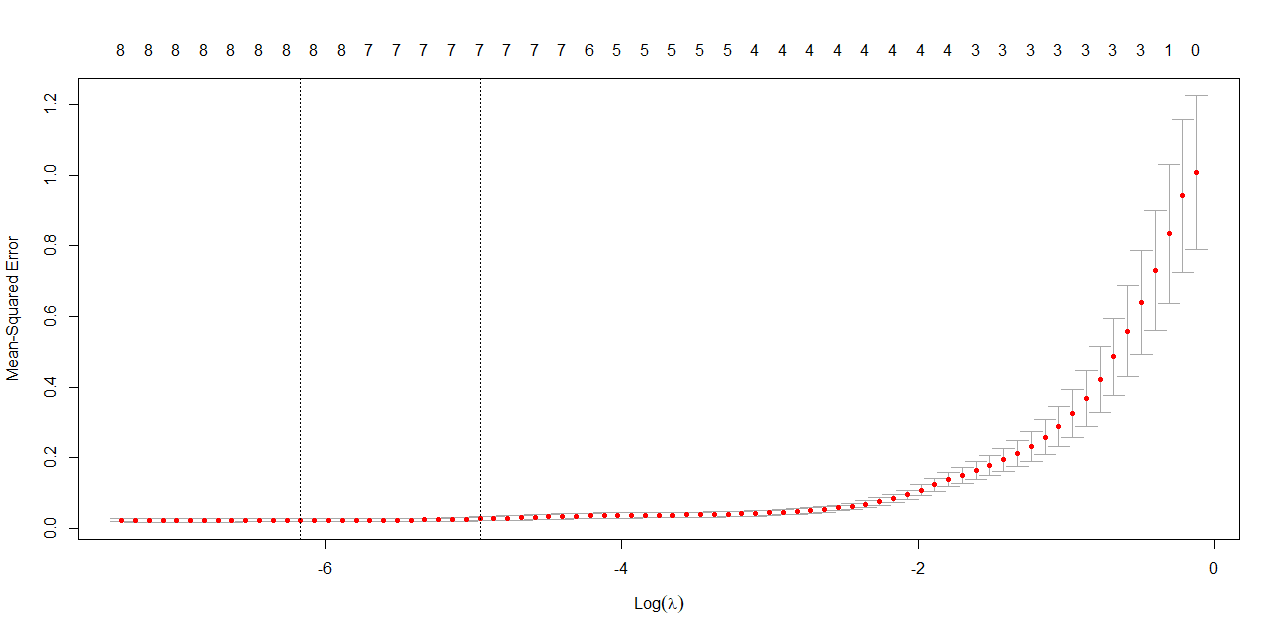
\includegraphics[scale = 0.26]{LASSORegression_Plot.png}\\
\hline
\end{tabular}
\end{table*}

\begin{table*}[ht]
\caption{Household Debt Auto Correlation}
\centering
\begin{tabular}{p{1.0\linewidth}}
\hline
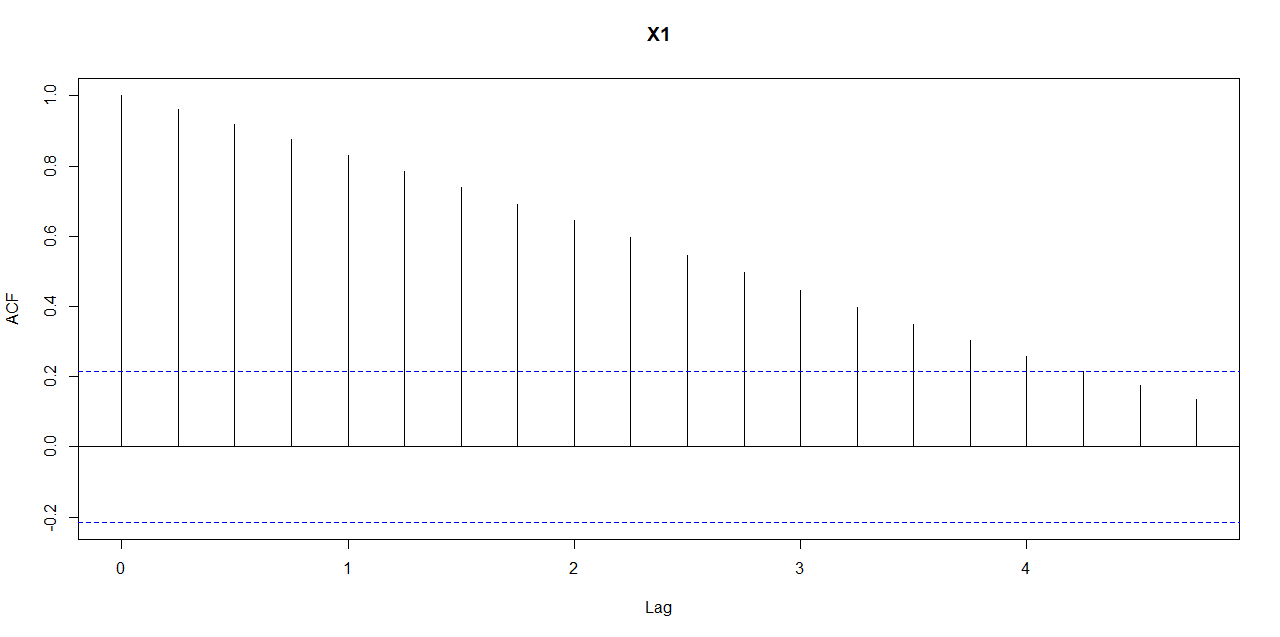
\includegraphics[scale = 0.26]{HouseholdDebtAutoCor.png}\\
\hline
\end{tabular}
\end{table*}



\begin{table*}[ht]
\caption{Microsoft Azure Machine Learning Experiment}
\centering
\begin{tabular}{p{1.0\linewidth}}
\hline
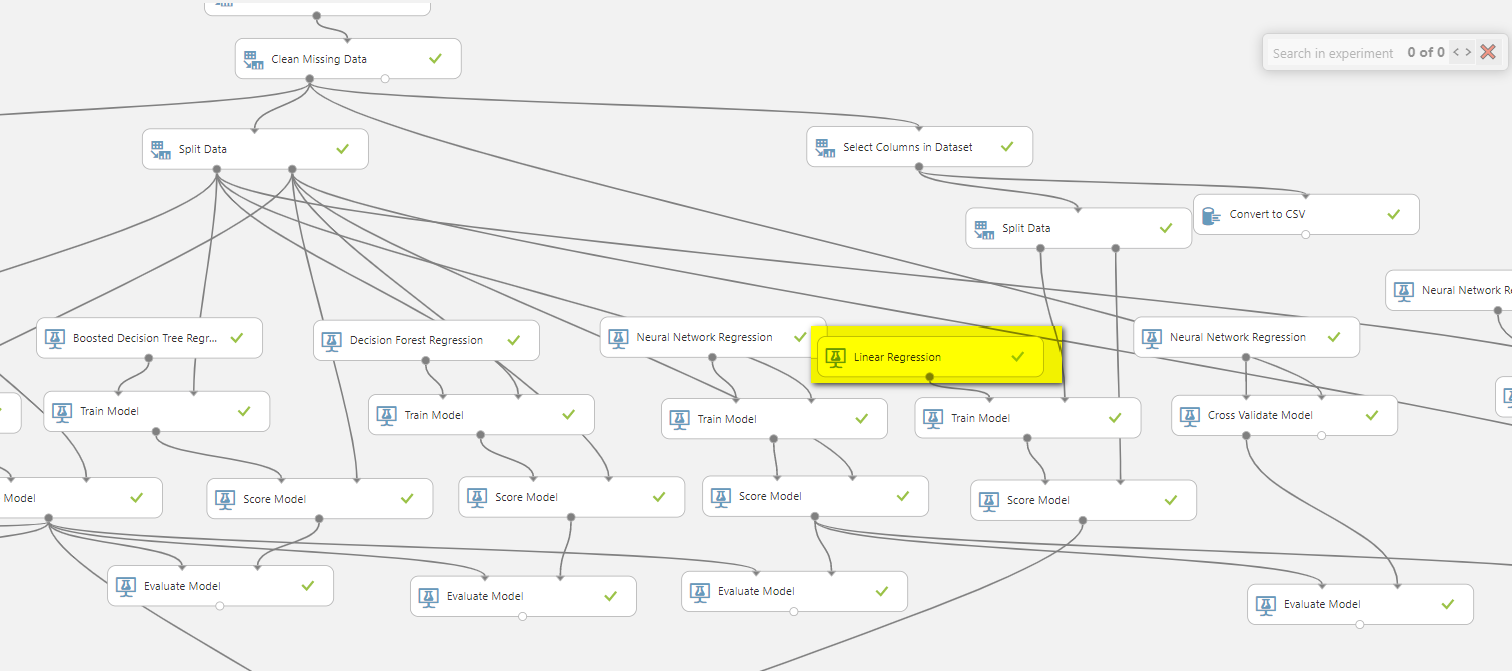
\includegraphics[scale = 0.46]{teamfed_azure_ml.png}\\
\hline
\end{tabular}
\end{table*}


\begin{table*}[ht]
\caption{Model Performance}
\centering
\begin{tabular}{p{1.0\linewidth}}
\hline
\includegraphics[scale = 0.46]{linreg.png}\\
\hline
\end{tabular}
\end{table*}

\end{appendix}


\begin{table*}[ht]
\caption{Source Code}
\centering
\begin{tabular}{p{0.3\linewidth}p{0.7\linewidth}}
\hline
Source Folder & Description \\
\hline
root folder & The README.md file in this directory contains information about the project\\
            & and team members. It also contains information about the project data sets\\
\hline
rcode & R source code used to generate plots to assist with variable selection. Please \\
      & see the README.md file in this directory.\\
\hline
spark\_scala\_importer & Scala Apache Spark code to import data into SQLite, clean \& transform data,\\
                       & and export to a CSV file used by Azure ML Studio. Please see the README.md\\
                       & file in this directory for setting up your IDE to compile the source code.\\
\hline
webapp                 & Angular and Bootstrap source code for web application. The Docker build files\\
                       & are also here.  Please see the README.md file in this directory.\\
\hline
\end{tabular}
\end{table*}



% \section{Research Methods}

% \subsection{Part One}

% Lorem ipsum dolor sit amet, consectetur adipiscing elit. Morbi
% malesuada, quam in pulvinar varius, metus nunc fermentum urna, id
% sollicitudin purus odio sit amet enim. Aliquam ullamcorper eu ipsum
% vel mollis. Curabitur quis dictum nisl. Phasellus vel semper risus, et
% lacinia dolor. Integer ultricies commodo sem nec semper.

% \subsection{Part Two}

% Etiam commodo feugiat nisl pulvinar pellentesque. Etiam auctor sodales
% ligula, non varius nibh pulvinar semper. Suspendisse nec lectus non
% ipsum convallis congue hendrerit vitae sapien. Donec at laoreet
% eros. Vivamus non purus placerat, scelerisque diam eu, cursus
% ante. Etiam aliquam tortor auctor efficitur mattis.

% \section{Online Resources}

% Nam id fermentum dui. Suspendisse sagittis tortor a nulla mollis, in
% pulvinar ex pretium. Sed interdum orci quis metus euismod, et sagittis
% enim maximus. Vestibulum gravida massa ut felis suscipit
% congue. Quisque mattis elit a risus ultrices commodo venenatis eget
% dui. Etiam sagittis eleifend elementum.

% Nam interdum magna at lectus dignissim, ac dignissim lorem
% rhoncus. Maecenas eu arcu ac neque placerat aliquam. Nunc pulvinar
% massa et mattis lacinia.
\end{document}
\endinput
%%
%% End of file `sample-sigconf.tex'.
